\documentclass[xcolor=dvipsnames]{beamer}
\usepackage{graphicx,epstopdf}
\usepackage{fancyhdr}
\usepackage{cite}
\usepackage{graphicx, epstopdf}
\usepackage{amsmath}
\usepackage{array}
\usepackage{epsfig}
\usepackage{amssymb}
\usepackage{subfigure}
\usepackage[ruled, lined,linesnumbered]{algorithm2e}
\usepackage{algorithmic}
\usepackage{tabularx}
\usepackage{rotating, boxedminipage}
\usepackage{rotating,multirow}
\usepackage{float}
\usepackage{wrapfig}
\usepackage{algorithm2e}
\usetheme{Boadilla}
\usecolortheme[named=Blue]{structure}
\setbeamertemplate{items}[square]
\setbeamertemplate{caption}[numbered]
\setbeamertemplate{caption}[small]
\usepackage[absolute,overlay]{textpos}
\newenvironment{reference}[2]{%
  \begin{textblock*}{\textwidth}(#1,#2)
     \bgroup\fontsize{6pt}{\baselineskip}\selectfont\color[RGB]{0,112,192}}{\egroup\end{textblock*}}

\begin{document}
    \title[SSCI]{A Hybrid Estimation of Distribution Algorithm with Differential Evolution for Global Optimization}
    \author[B. Dong, A. Zhou, G. Zhang]{Bing Dong, Aimin Zhou, Guixu Zhang}
    \institute[ECNU]{East China Normal University, Shanghai, China}
    \logo{\includegraphics[height=0.5cm,width=3.0cm]{university-logo-ecnu}\vspace{230pt}}
    \date{December 2016}
    \begin{frame}
        \titlepage
    \end{frame}
    \setbeamertemplate{section in toc}[square]
    \begin{frame}
        \frametitle{Outline}
        \tableofcontents
    \end{frame}

    \section{Background}
    \begin{frame}
      \frametitle{Outline for Section \thesection}
      \tableofcontents[currentsection]
    \end{frame}

    \begin{frame}
    \frametitle{Definition}
    The box-constrained continuous global optimization can be stated in the following:
    \begin{equation}
    \begin{array}{rl}
    \mbox{min} & f(x)\\
    \mbox{s.t} & x\in[a_i,b_i]^n
    \end{array}
    \label{MOP}
    \end{equation}

    \begin{itemize}
    \item $x=(x_1, x_2, \cdots, x_n)^T\in{R^n}$ is a decision vector
    \item $[a_i, b_i]^n$ is the search space
    \item $f:R^n\to{R}$ is the objective function
    \end{itemize}
    \end{frame}


    \begin{frame}
    \frametitle{Differential Evolution(DE)}

    DE is a simple but powerful optimization algorithm. Classical DE algorithm consists of three steps:
    \begin{itemize}
    \item mutation: Utilize mutation operator to generate mutant vector.
    \item crossover: Utilize crossover operator to generate trial vector.
    \item selection: Target vector and trial vector competes to enter the next generation.
    \end{itemize}

%    \begin{columns}
%        \begin{column}{0.5\textwidth}
%        \begin{figure}[H]
%            \graphicspath{{figs/}}
%            \includegraphics[width=0.9\textwidth]{de.png}
%            \caption{The algorithm framework of DE}
%        \end{figure}
%    \end{column}
%    \begin{column}{0.5\textwidth}
%    \begin{itemize}\small
%    \setlength\itemsep{0em}
%      \item $N$ is the population size, and $D$ is the dimension of the target vector.
%      \item At each generation $G$, a mutant vector $v_{i,G}$ is obtained by mutation. $F$ is the scaling factor, $r1, r2, r3$ are mutually different integers randomly selected from $[1,N]$.
%      \item The trial vector $u_{i,j,G}$ is generated by combing $v_{i,G}$ and $x_{i,j,G}$. $rand_j(0,1)\in[0, 1]$ is a uniformly distributed random number, and $j_{rand}$ is a random integer between $j$ and $D$. $CR$ is the controlling parameter.
%      \item $u_{i,G}$ and $x_{i,G}$ compete to enter the next generation in accordance with the objective function value.
%    \end{itemize}
%    \end{column}
%    \end{columns}

    \end{frame}

    \begin{frame}
    \frametitle{Estimation of Distribution Algorithm(EDA)}
    EDA is a recent stochastic optimization algorithm which mainly includes three steps:
    \begin{itemize}
    \item modeling: Build a probabilistic model.
    \item sampling: Generate individuals according to the built probabilistic model.
    \item selection: Select individuals from the generated individuals and parent population to the next generation.
    \end{itemize}
%    \begin{columns}
%        \begin{column}{0.5\textwidth}
%        \begin{figure}[H]
%            \graphicspath{{figs/}}
%            \includegraphics[width=0.9\textwidth]{eda.png}
%            \caption{The algorithm framework of DE}
%        \end{figure}
%    \end{column}
%    \begin{column}{0.5\textwidth}
%    \begin{itemize}\small
%    \setlength\itemsep{0em}
%    \item $t$ is the generation counter.
%    \item $Pop(t)=\{x^1,x^2, \cdots x^N\}$ is the population at generation $t$.
%    \item $Q$ is a new solution set sampled from the probabilistic model.
%    \end{itemize}
%    \end{column}
%    \end{columns}
    \end{frame}


    \section{Our algorithm}
    \begin{frame}
      \frametitle{Outline for Section \thesection}
      \tableofcontents[currentsection]
    \end{frame}

    \begin{frame}
    \frametitle{DE-EIG}
    DE-EIG is novel DE which utilize eigenvector to rotate the original coordinate system. It is significant to extract the statistical information form the population.
    \begin{block}{Crucial work:}
    \begin{itemize}
    \item crossover in a rotated coordinate system
    \item utilize a appropriate parameter to control the crossover in the original coordinate system or the rotated coordinate system
    \end{itemize}
    \end{block}
%    \begin{columns}
%        \begin{column}{0.5\textwidth}
%        \begin{figure}[H]
%            \graphicspath{{figs/}}
%            \includegraphics[width=0.8\textwidth]{de-eig.png}
%            \caption{The algorithm framework of DE-EIG}
%        \end{figure}
%    \end{column}
%    \begin{column}{0.5\textwidth}
%    As traditional DE operates crossover in the original coordinate, it is inevitable to lose some statistics information. DE-EIG based on the eigenvectors makes the crossover rotationally invariant by transform the coordinate system of the individuals in the population.
%    \end{column}
%    \end{columns}
    \end{frame}

    \begin{frame}
    \frametitle{DE/EDA}
    DE/EDA is a algorithm combining DE and EDA.

    Its main work:
    \begin{itemize}
    \item combine the differential information from DE and global information from EDA
    \item make a parameter to control the sampling of EDA
    \end{itemize}
%    \begin{columns}
%        \begin{column}{0.5\textwidth}
%        \begin{figure}[H]
%            \graphicspath{{figs/}}
%            \includegraphics[width=0.8\textwidth]{deeda.png}
%            \caption{The algorithm framework of DE/EDA}
%        \end{figure}
%    \end{column}
%    \begin{column}{0.5\textwidth}
%    CRP is utilized to control the offspring generation by DE or EDA. DE/EDA utilized the global information extracted by EDA and the differential information exploited by DE to obtain promising solutions.
%    \end{column}
%    \end{columns}
    \end{frame}

    \begin{frame}
    \frametitle{EDA/DE-EIG}
    Based on the framework of DE/EDA, we propose EDA/DE-EIG.

    Our thoughts:
    \begin{enumerate}
    \item Import DE-EIG to improve the sampling of EDA.
    \item Utilize a random parameter to control the resource allocations of DE-EIG and EDA.
    \item Expensive local search is applied to refine the solutions further more.
    \end{enumerate}

    \end{frame}

    \begin{frame}
    \frametitle{Algorithm Framework}
%    \begin{columns}
%    \begin{column}{0.5\textwidth}
    \begin{figure}[H]
    \graphicspath{{figs/}}
    \includegraphics[width=0.4\textwidth]{deeda-eig.png}
    \caption{The algorithm framework of EDA/DE-EIG}
    \end{figure}
%    \end{column}
%    \begin{column}{0.5\textwidth}
%    Based on the framework of DE/EDA, DE-EIG is imported to improve the sampling in the algorithm. For Converage($\theta, G, G_e$) at line 16, it is essential to judge whether to operate expensive local search.
%    \end{column}
%    \end{columns}
    \end{frame}



    \section{Experiment results}
    \begin{frame}
      \frametitle{Outline for Section \thesection}
      \tableofcontents[currentsection]
    \end{frame}

    \begin{frame}
    \frametitle{Compared algorithms and \par experimental setting}
    In this paper, EDA/DE-EIG is compared with JADE and DE/EDA on the first 13 test instances form YYL test instances.

    \begin{itemize}\small
    \setlength\itemsep{0em}
    \item The dimension of the population is 30. All algorithms are run independently 50 times and stopped after 450,000 function evaluations.
    \item JADE: $N=150, p=0.05, c=0.1, F=0.5$ and $CR=0.9$.
    \item DE/EDA: $N=150, F=0.5$ and $CRP=0.9$.
    \item EDA/DE-EIG: $N=150, CRP=0.5, f=0.5, CR = 0.6, P=0.5, \theta=0.1$.
    \end{itemize}

    All the algorithms are implemented by Matlab and executed at the same computer.
    \end{frame}

    \begin{frame}
    \begin{figure}[H]
        \graphicspath{{figs/}}
        \includegraphics[width=0.8\textwidth]{tab1-1.jpg}
    \end{figure}
    \end{frame}

    \begin{frame}
    \begin{figure}[H]
        \graphicspath{{figs/}}
        \includegraphics[width=0.8\textwidth]{tab1-2.jpg}
    \end{figure}
    \end{frame}

    \begin{frame}
    \begin{figure}[H]
        \graphicspath{{figs/}}
        \includegraphics[width=0.8\textwidth]{tab1-3.jpg}
    \end{figure}
    \end{frame}

    \begin{frame}
    \begin{figure}
    \centering
    \graphicspath{{figs/}}
    \subfigure[$f$1]{\includegraphics[ width=0.25\textwidth]{f1.eps}}
    \subfigure[$f2$]{\includegraphics[ width=0.25\textwidth]{f2.eps}}
    \subfigure[$f3$]{\includegraphics[ width=0.25\textwidth]{f3.eps}}
    \subfigure[$f4$]{\includegraphics[ width=0.25\textwidth]{f4.eps}}
    \subfigure[$f5$]{\includegraphics[ width=0.25\textwidth]{f5.eps}}
    \subfigure[$f7$]{\includegraphics[ width=0.25\textwidth]{f7.eps}}
    \caption{The mean function value versus on $f1-f7$ except $f6$.}
     \label{fig1}
    \end{figure}
    \end{frame}

    \begin{frame}
    \begin{figure}
    \centering
    \graphicspath{{figs/}}
    \subfigure[$f8$]{\includegraphics[ width=0.25\textwidth]{f8.eps}}
    \subfigure[$f9$]{\includegraphics[ width=0.25\textwidth]{f9.eps}}
    \subfigure[$f10$]{\includegraphics[ width=0.25\textwidth]{f10.eps}}
    \subfigure[$f11$]{\includegraphics[ width=0.25\textwidth]{f11.eps}}
    \subfigure[$f12$]{\includegraphics[ width=0.25\textwidth]{f12.eps}}
    \subfigure[$f13$]{\includegraphics[ width=0.25\textwidth]{f13.eps}}
    \caption{The mean function value versus on $f8-f13$}
     \label{fig2}
    \end{figure}
    \end{frame}

    \begin{frame}
    According to figure~\ref{fig1} and figure~\ref{fig2}, the following conclusions are obtained:
    \begin{enumerate}
    \item obtain best results on 8 out of 12 test instances
    \item better than DE/EDA except $f7$ and $f8$
    \item has a similar performance in comparison with JADE
    \end{enumerate}

    \end{frame}

    \section{Conclusions and future work}
    \begin{frame}
      \frametitle{Outline for Section \thesection}
      \tableofcontents[currentsection]
    \end{frame}

    \begin{frame}
    \frametitle{Conclusions}
    \begin{enumerate}
    \item DE/EDA is a promising algorithm framework utilizing global and local information.
    \item DE-EIG is significant to improve the sampling.
    \item EDA/DE-EIG has a impressive performance comparing with JADE and DE/EDA.
    \end{enumerate}
%    DE/EDA is a promising method that utilizes both the the global and local information for global optimization. However, the potential improvement of the performance of this algorithm has not been exploited furthermore.
%    \par
%     In this paper, an improved DE, DE-EIG, is imported to combine with EDA, bringing an impressive improvement on the performance. DE-EIG is beneficial to utilize the statistics information of the population to accelerate the convergence. And expensive local search is applied to improve the performance further.
%
%     The experimental results have shown the distinct advantages of the proposed method, named as EDA/DE-EIG, in comparison with two state-of-art algorithms JADE and DE/EDA.
    \end{frame}

    \begin{frame}
    \frametitle{Future work}
    The results reported in this paper is preliminary and there are several ways to improve the algorithm performance. The future work includes:
    \begin{itemize}
    \item simplify the algorithm framework of EDA/DE-EIG
    \item investigate the resources allocation of DE-EIG and EDA
    \end{itemize}
%     Firstly, the algorithm framework of EDA/DE-EIG can be simplified. Secondly, it is worth to investigate how to allocate the computational resources to both DE-EIG and EDA.
    \end{frame}


    \section*{thx}
        \begin{frame}
        \begin{center}
        %\structure
        \fontsize{60pt}{\baselineskip}\selectfont \structure{Thanks!}
        \end{center}
        \begin{reference}{0mm}{80mm}
        \begin{itemize}
        \item  B. Dong, A. Zhou, and G. Zhang, A Hybrid Estimation of Distribution Algorithm with Differential Evolution for Global Optimization, 2016 IEEE Symposium Series on Computational Intelligence (SSCI), 2016.
        \end{itemize}
        \end{reference}
        \end{frame}
\end{document}
